\emph{This chapter has been published as part of~\textcite{VanDenKerchove2024}}

\section{Introduction}
\todo{mention cble and wcble in methods}

\textcite{Arico2014} observed higher variability in single-trial P3 peak
latencies relative to stimulus onset during covert VSA compared to overt VSA.
This latency variability contributes to reduced covert VSA decoding performance.
While they proposed an analysis and performance prediction method, they did not provide a
decoding solution.
They suggested that compensating for latency jitter could enhance covert VSA
decoding, but did not actually verify this hypothesis directly.
Additionally, \cite{Hardiansyah2020} developed a classifier for
covert VSA ERPs, exploiting single-trial latency features in combination with
amplitude features for classification with a support vector machine.
They demonstrated the positive influence of single-trial ERP component latency
features on covert VSA inference, yet did not attempt to correct the amplitude
features for these latencies.
\todo{Should we already mention Frenzel here?}
\textcite{Frenzel2011} introduced a similar protocol to our split VSA
setting.
They showed that it is possible to perform split VSA and that, in this
case, visuospatial attention and gaze direction can separately be decoded using
classical ERP techniques.
To the best of our
knowledge, this is the sole study that investigated split attention in ERP-based BCIs.
However, \textcite{Frenzel2011} considered their interface only for the case
where the user actively intends to select both targets determined by the gaze
and the VSA.
In the split VSA setting considered in our work, we rather instruct the participant to ignore
the distractor and only attend the cued target, since we are interested in
decoding the visuospatial attention only.
\todomvh{avoid overlap. it seems already explained in previous sentences. The reader can find details in
  [6].}

frenzel
\todo{part about split attention etc from chapter on covert alignment to here}

\section{Materials \& methods}

\subsection{Data collection}
We evaluate our approach on the
publicly available BNCI2014-009 dataset~\cite{Aloise2012a} and one specifically recorded for this study, designed to
probe different modalities of covert VSA.
\todomvh{first explain BNCI2014-009 using fig. 6.1 or revert the announcement
in the previous sentence.}

\subsubsection{CVSA-ERP dataset}
\label{sec:covert-align/stimulation}

We recorded a dataset to validate our approach.
The Covert Visuospatial Attention ERP (CVSA-ERP) dataset
consists of 15 participants, mean age $26.34\pm3.04$ years.
This study was approved by the Ethics Commission of University Hospital Leuven
(S62547).
Each subject performed different VSA conditions (overt, covert and split),
illustrated in Figure~\ref{fig:interface} (top row).
Using a hexagonal layout interface, similar to the visual Hex-o-Spell proposed
by \cite{Treder2010}, we present six flashing targets (without letters or
symbols) to the participant while the EEG, electrooculogram (EOG), and the
participant's eye gaze using eye tracking were recorded.
The VSA conditions described in the first row of Figure~\ref{fig:interface} are
considered.
\begin{figure*}
  \bigskip
	\begin{subfigure}{\linewidth}
		\caption{}
		\label{fig:interface}
		\includegraphics[width=\linewidth]{figures/covert_align/figure3a.pdf}
	\end{subfigure}

	\bigskip
	\bigskip
	\begin{subfigure}{\linewidth}
		\caption{}
		\label{fig:erps}
		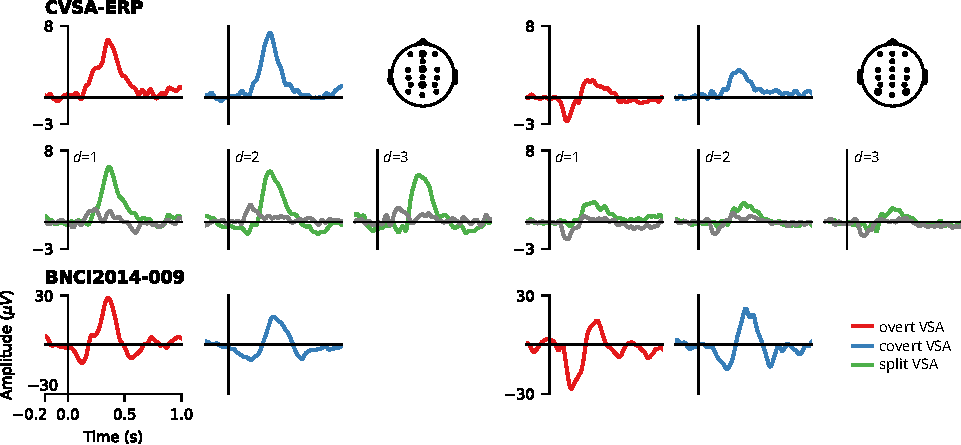
\includegraphics[width=\linewidth]{figures/covert_align/figure3b.pdf}
	\end{subfigure}%

	\caption{
		\subref{fig:interface} Interfaces and visuospatial attention (VSA)
    conditions in the CVSA-ERP and BNCI2014-009 datasets.
		In the CVSA-ERP oddball BCI interface, screen targets are intensified one after
    the other in pseudorandom order while the participant can either pay overt,
    covert, or split VSA to the cued target.
		In the BNCI2014-009 overt VSA interface, entire rows and columns are
		intensified at once. In its covert counterpart,
		groups of 6 letters are intensified one after the other, partly relying on
    feature attention.
		\subref{fig:erps} Contrast between target (color) and non-target, and
    distractor (gray) and non-target grand average event-related potentials per VSA condition and dataset.
    Overt VSA yields a strong modulation of the N1 component in both datasets;
    the P3 amplitude decreases with the degree of split VSA.
    In split VSA, N1 and P2 are more prominently evoked by the distractor,
    while the P3 is evoked by the target.
	}
\end{figure*}

In contrast to the protocol proposed by \cite{Frenzel2011}, split VSA was
performed by instructing the participant to attend the intensifications of the
cued target, and ignore the intensifications of the distractor target.
Since we assume there will be an effect depending on the distance between
attended target and the distractor, we discern three split VSA sub-conditions:
the distractor is either clockwise or counterclockwise directly next to the
attended target ($d=1$), there is one other target between the attended target and
the distractor ($d=2$), or the distractor is opposite to the intended target
($d=3$).

EEG for the CVSA-ERP dataset was recorded using a SynAmps RT amplifier
(Compumedics Neuroscan, Australia) at 2048Hz and 62 Ag/AgCl active electrodes arranged in the
international 10-10 layout fitted to a standard electrode cap (EASYCAP GmbH,
Germany), with electrodes located at AFz and FCz as ground and reference respectively.
Using electrolyte gel, electrode impedances were brought below 5k$\Omega$.
Electrodes TP9 and TP10, used for off-line re-referencing, were directly
attached to the skin using stickers for better contact.
The power line frequency in Belgium is 50 Hz.
Participant's eye gaze was registered using an EyeLink 1000 Plus eye tracker (SR Research,
Canada) in non-fixation mode.

Participants signed the informed consent form and were seated at a distance of
60 cm before a CRT-emulating monitor (VPixx
Technologies, Canada) operating at a refresh rate of 120Hz, displaying 6
circular white targets with a diameter of 4.15° visual angle and laid out on a hexagon
with a radius of 12.28° of visual angle centered on the midpoint of the screen,
conforming to the interface proposed by \textcite{Treder2010}
(Figure~\ref{fig:layout_targets})\todo{figure interface in four panels and
update all refs below}.
A hexagonal layout interface with an empty center and a low number of targets
counteracts target crowding and, as long as the subject’s gaze is within the hexagon of
targets, no other target can be between the subject’s gaze and a covertly
attended target.
Targets are full-contrast white and were intensified by scaling them to a
larger size (5.60° of visual angle, Figure~\ref{fig:layout_intense}) instead of changing the contrast to avoid Troxler-fading\footnote{The optical illusion of disappearing unchanging stimuli
experienced when visually fixating~\cite{Troxler1804}.}~\cite{Treder2010} in the
peripheral visual field.
Stimuli were presented using PsychopPy (version 2023.1.3)~\cite{Peirce2019}.
\todo{figures}
\todo{figures from ethical protocol Lille}

The participant was instructed to press the space bar when ready for a block
of stimulations.
Then, one target was indicated as the cue and the participant
was instructed to count the number of intensifications of the cued target
during the following block of stimulations.
After pressing the space bar again, a blue crosshair appeared, and the subject
was instructed to fixate their gaze on the blue crosshair for the duration of
the stimulation block (Figure~\ref{fig:layout_cross_overt} and Figure~\ref{fig:layout_cross_covert}).
The position of this crosshair determined the VSA condition for this trial:
overt VSA when the crosshair was at the same location as the cued target,
covert VSA when the crosshair appeared in the center of the screen, and split
VSA when the crosshair appeared on a different target than the cued one.
After pressing the space bar again and a delay of 5 seconds, the stimulation block
starts.

All targets were intensified for a duration of 100 ms, in pseudorandom order.
The inter-stimulus-interval (ISI), the time between the onsets of subsequent intensifications,
was variable and consisted of a fixed 300ms interval (of which 100ms with an intensified target onscreen)
with 200ms uniform jitter added, resulting in an ISI
between 200 and 400 ms.
\Acp{isi} were jittered to counteract steady-state effects and residue in averaging. A
longer \ac{isi} will increase component amplitude and aid in counteracting temporal
autocorrelation for a higher statistical test precision.
In a block of stimulations, each target was intensified a pseudorandom number of times between 10 and 15.
This led to stimulation blocks with an average duration of 26.25 seconds. After a block of stimulations, an
input prompt appeared to enter the mentally counted number of intensifications.
After inputting this number, the subject was allowed to pause until pressing the space bar again.
In total, six blocks were presented for overt VSA, six blocks for covert VSA, 12 blocks for
split ($d=1$) VSA, 12 blocks for split ($d=2$) VSA and 6 blocks for split
($d=3$) VSA, covering all possible combinations of VSA conditions, cued targets and
crosshair locations.

The experiment started with five non-recorded practice stimulation blocks, one for
each of the 5 VSA conditions.
During these practice blocks, the participant received feedback about their gaze
position and counting accuracy.
Counting the instructions and the participant's response to the
input prompts, a block lasted about 30
seconds. In sum, the experiment featured approximately 45 minutes of
stimulation time.
After blocks 14 and 28, the participant was allowed to take a longer break.
Including these longer breaks, the experiment lasted approximately one hour.

\subsubsection{BNCI2014-009 dataset}
The
BNCI2014-009\footnote{\url{https://bnci-horizon-2020.eu/database/data-sets}}
dataset~\cite{Aloise2012a} was used in the analysis performed
in \cite{Arico2014}.
It contains data from 10 subjects (median age $24.5\pm1.9$
years)  that performed two spelling tasks illustrated in the second row of
Figure~\ref{fig:interface}: using the P3 Matrix speller
interface to exploit overt VSA, and the GeoSpell covert VSA interface.
To use the GeoSpell interface, the participant gazes at the fixation point at the
center of the screen, while groups of characters flash simultaneously in a
circular layout around the fixation point.
The user directs their visuospatial attention to the location where the intended letter is expected
to appear, and when it does, a P3 ERP component is expected to be evoked.
This results in a specific setting where both visuospatial attention and
feature attention (the attended letter) are exploited.
For a detailed description of the paradigm and dataset, we refer
to \cite{Aloise2012a}.

\subsection{Data processing and analysis}
\subsubsection{Preprocessing}
Analysis was performed using Python and the MNE software package (version
1.3.1)~\cite{Gramfort2013}.
All datasets were band-pass filtered between 0.1Hz and 20Hz with a 4th-order Butterworth filter.
Bad channels in the data were automatically detected using the RANSAC
method~\cite{Fischler1981} and rejected.
The recorded EEG was re-referenced
offline to the average of the mastoid electrodes TP9 and TP10.
Next, the EEG signals were corrected for eye movement artifacts using an
Independent Component Analysis (ICA).
Since we have access to EOG data for the CVSA-ERP dataset components correlating
significantly with the EOG were rejected.
For the BNCI2014-009 dataset, ICA components were manually rejected.
Finally, the EEG signal is divided into epochs ranging from 100ms before stimulus onset to 700ms after stimulus onset and down-sampled to 128Hz.
In both datasets, only 16 channels were kept for
analysis (Fz, FCz, Cz, CPz, Pz, Oz, F3, F4, C3, C4, CP3, CP4, P3, P4, PO7 and
PO8).

\subsubsection{Decoders}
We will compare \ac{wcble} and \ac{cble} as described in
Section~\ref{sec:wcble/methods}, with their base classifier and tLDA and with
Riemannian Geometry
approaches that rely on spatial covariance as features.
Together with tLDA, Riemannian Geometry generally reaches state-of-the-art decoding
performance~\cite{Lotte2018}.
We implemented two Riemannian Geometry pipelines.
The first one estimates shrunk covariances from the ERPs filtered with 6 XDAWN
filters, projects these covariances to a tangent space and classifies the
result using $L_2$-regularized logistic regression
(XDAWNCov-TS-LR)~\cite{Cecotti2017}.
Secondly, we adopt the pipeline from \cite{Aydarkhanov2020}, since their work shows
favorable performance in the presence of single-trial ERP latency jitter.
Shrunk spatial covariance matrices are estimated from epochs that are
augmented by concatenating the average target and average non-target ERP as
extra channels, projected to tangent space and classified using
$L_2$-regularized logistic regression (ERPCov-TS-LR).

To evaluate performance, 6-fold cross-validation without shuffling was performed for both
datasets.
At each fold, classifiers were trained on five target selection blocks (300
epochs) and tested on one block (60 epochs) without overlap for CVSA-ERP.
For each subject and run in the BNCI2014-009 dataset, classifiers
were trained on five symbol selections (480 epochs) and tested on one symbol
selection (96 epochs) without overlap at each fold.
A window ranging from 0ms to 600ms after stimulus onset was used for CBLE and WCBLE.
With epochs ranging from -100ms to 700ms relative to stimulus onset, this
allows for extracting latencies ranging from -100ms to +100ms.



\section{Results}

\subsection{BCI decoding performance}
\label{sec:block_accuracy}

We evaluated the BCI decoding performance in a single-trial classification
experiment, as well as in a target selection experiment reflecting BCI
operation.

Figure~\ref{fig:single_trial_roc_auc_diff} shows a comparison of areas under the
Receiver Operating Characteristic curve (ROC-AUC) for all pairs of tLDA, CBLE
and WCBLE for single-trial classification to investigate the contributions of
CBLE and WCBLE relative to their first-stage classifier tLDA.
For this evaluation, epochs were rejected when the peak-to-peak amplitude
exceeded 800$\mu V$ and, for the CVSA-ERP dataset, if the user's gaze differed more than
10 degrees of visual angle from the fixation crosshair.
\begin{figure}
  \bigskip
	\begin{subfigure}{\linewidth}
		\caption{}
		\label{fig:single_trial_roc_auc_diff}
		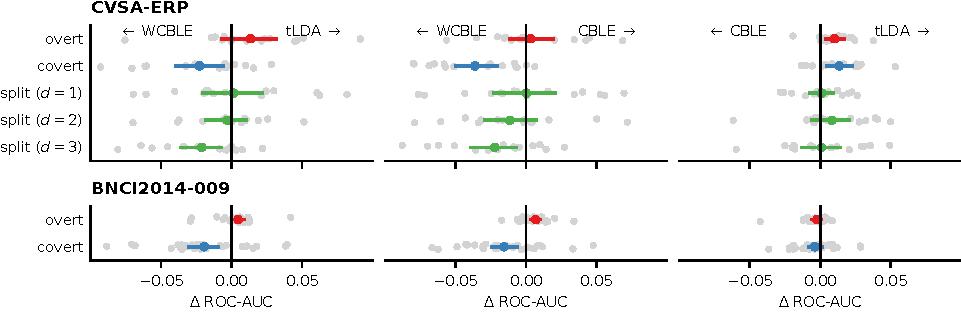
\includegraphics[width=\linewidth]{figures/covert_align/figure4a.pdf}
	\end{subfigure}

	\bigskip

	\begin{subfigure}{\linewidth}
		\caption{}
		\label{fig:block_evaluation}
		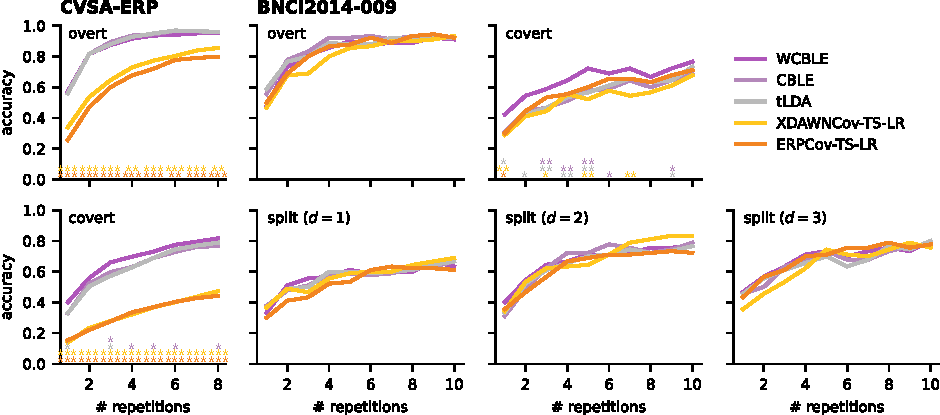
\includegraphics[width=\linewidth]{figures/covert_align/figure4b.pdf}
	\end{subfigure}
	\caption{
		\subref{fig:single_trial_roc_auc_diff} Difference in cross-validated
    single-trial classification receiver operating characteristic curve ($\Delta$ROC-AUC)
    between Classifier-based Latency Estimation (CBLE), Woody
    CBLE (WCBLE),	and their first-stage classifier (tLDA).
    95\% confidence intervals were determined using $k=1000$ bootstrapping.
    Our proposed WCBLE decoder outperforms tLDA and CBLE for covert and split
		($d=3$)	visuospatial attention (VSA). CBLE scores on par with tLDA.
		\subref{fig:block_evaluation} Cross-validated target selection accuracy for
    all decoders plotted n function of the number of test repetitions in
    different VSA conditions. Significance was determined using one-sided
    (WCBLE $>$ other) Wilcoxon rank-sum tests using False Discovery Rate correction
    ($*= p<0.05$, $**=p<0.01$, $***=p<0.001$). WCBLE generally achieves highest
    covert VSA target selection accuracy.}
\end{figure}
Wilcoxon signed-rank tests controlled for multiple comparisons by Benjamini
and Hochberg's False Discovery Rate procedure (FDR) revealed that
for the BNCI2014-009 dataset, WCBLE significantly outperformed tLDA
($\Delta\mathrm{ROC-AUC} = 0.019$, $p=0.004$) and CBLE
($\Delta\mathrm{ROC-AUC} = 0.016$, $p=0.036$) for covert VSA
but was significantly outperformed by tLDA in overt VSA decoding
($\Delta\mathrm{ROC-AUC}=-0.004$, $p=0.040$).
For the CVSA-ERP dataset, WCBLE
also achieved significantly better covert VSA performance than tLDA ($\Delta\mathrm{ROC-AUC}
	= 0.023$, $p=0.041$) and CBLE ($\Delta\mathrm{ROC-AUC}
	= 0.036$, $p=0.024$) .
We found no significant difference in WCBLE performance over tLDA in the split
VSA conditions in the CVSA-ERP dataset, but results show a clear trend of
increase in WCBLE performance over tLDA and CBLE as $d$ increases
CBLE failed to significantly outperform its first-stage classifier tLDA in all
evaluated VSA conditions.
Table~\ref{tab:single_trial_full} reports all single-trial classification scores for all considered models, datasets
and conditions.
\todo{table?}

Figure~\ref{fig:block_evaluation} shows the cross-validated BCI selection
accuracy on the BNCI2014-009 and the CVSA-ERP dataset for all investigated
decoders.
Accuracy was determined by, for each block, selecting the character with the
highest (stage-two if applicable) classifier score and comparing it to the cued target.
Significance was calculated using one-sided Wilcoxon rank-sum tests ($p=0.05$)
corrected for FDR over decoders.
For this evaluation, no epochs were rejected to keep the trial-based structure of BCI
operation intact.
For all datasets and VSA conditions, CBLE scores approximately on par with tLDA.
Yet, WCBLE yields an improved decoding accuracy for covert VSA in both
datasets, which is greatest for smaller numbers of repetitions and
decreases as the number of repetitions increases.
This covert VSA accuracy increase over tLDA is significant in the BNCI2014-009 dataset
for 1 and 3 repetitions and in CVSA-ERP for 1-5 and 10 repetitions.
Furthermore, while we reported a relative decrease in single-trial ROC-AUC for
WCBLE in overt VSA, this does not seem to result in a consistent decrease in target
selection accuracy.
No significant increase of WCBLE over other methods was found in split VSA.
While Riemannian methods are significantly outperformed by tLDA, CBLE and WCBLE
in the BNCI2014-009 dataset, they perform approximately on par with tLDA and
WCBLE in CVSA-ERP.

Overall, we observed a 5.10\%pt. accuracy increase with WCBLE over
tLDA for covert VSA in the BNCI2014-009 dataset and 5.55\%pt. in the CVSA-ERP dataset.
These results compare to the performance gain in \cite{Zisk2022}.
They observed a 5.63\%pt. accuracy increase with 1-10 selection repetitions over
step-wise Linear Discriminant Analysis  (SWLDA) for 6 ALS patients, whose SWLDA
performance also suffered from jitter.
Note that interpretation of this comparison may be challenging due to differences in
interface design (number of targets, \ac{isi}), subject population,
EEG recording procedure and available training data.


\subsection{Gaze-independence through cross-condition transfer}
\label{sec:cross_results}
To further back our claim of gaze-independence in the case where eye motor
control cannot be assumed, we evaluate our proposed decoder in a transfer
learning setting between VSA conditions.
While performing covert attention requires gaze redirection for each target
selection, performing covert or split VSA continuously still requires
sustained gaze fixation, which might not be possible for some patients that
could benefit from such an application.
Studying the transfer between conditions simulates what happens
when the user performs different VSA conditions throughout the
experimental session.
Furthermore, if our decoder performs well in transfer-learning settings,
it must capture some information about the ERP responses that is independent of
the VSA condition, and hence does not depend on gaze redirection to perform
these conditions.
We introduce an additional setting of interest here, namely on a combination of VSA
conditions, which represents those cases where patients cannot
redirect their gaze and hence can be in any one of the VSA conditions depending on the
target they attend.
For BNCI2014-009, this is implemented as an equal mix of overt and
covert VSA, for CVSA-ERP the combined condition represents an equal mix of overt,
covert and split VSA, disregarding parameter $d$.

Figure~\ref{fig:covert_cross_eval} and Figure~\ref{fig:aloise2012_cross_eval} show
the pair-wise differences in area under the ROC curve ($\Delta$ROC-AUC)
between the investigated decoders.
In this evaluation, bad epochs were rejected as in Section~\ref{sec:block_accuracy}.
\begin{figure*}
  \bigskip
	\begin{subfigure}{\linewidth}
		\caption{}
		\label{fig:covert_cross_eval}
		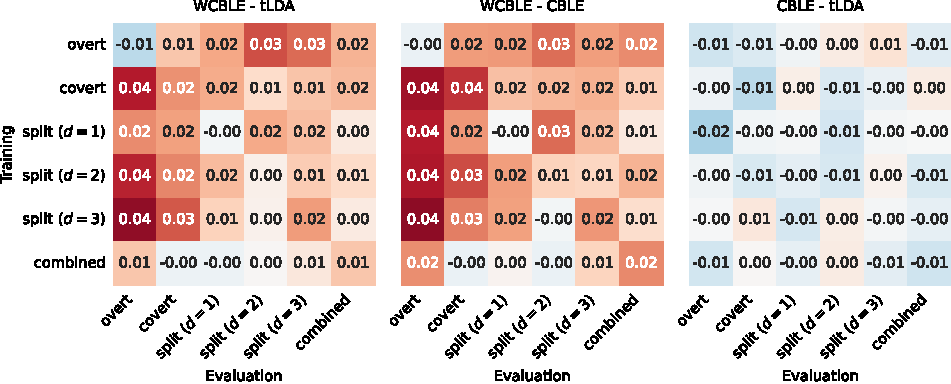
\includegraphics[width=\linewidth]{figures/covert_align/figure5a.pdf}
	\end{subfigure}

	\bigskip
	\bigskip

	\begin{subfigure}[c]{.48\linewidth}
		\caption{}
		\label{fig:aloise2012_cross_eval}
		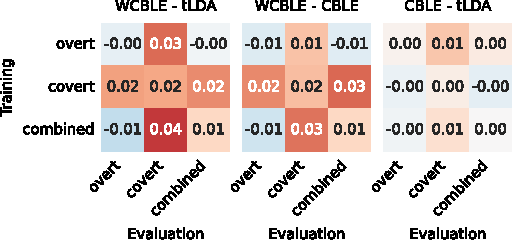
\includegraphics[width=\linewidth]{figures/covert_align/figure5b.pdf}
	\end{subfigure}\hfill%
	\begin{subfigure}[c]{.48\linewidth}
		\caption{}
		\label{fig:jitter}
		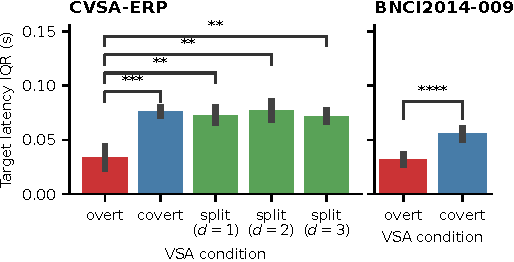
\includegraphics[width=\linewidth]{figures/covert_align/figure5c.pdf}
	\end{subfigure}

	\caption{
		\subref{fig:covert_cross_eval},\subref{fig:aloise2012_cross_eval}
    Difference in cross-validated area under the receiver
		operating characteristic curves between Classifier-based Latency Estimation
    (CBLE) and Woody CBLE (WCBLE) across conditions for the CVSA-ERP and
    BNCI2014-009 datasets respectively.
    A decoder is each	time trained on a visuospatial attention (VSA) condition
    and tested on all VSA conditions.
    WCBLE yields an improvement in most
		non-overt VSA settings, indicating it is more invariant to eye gaze than
    CBLE and tLDA.
		\subref{fig:jitter} Jitter characterized as the inter-quartile range (IQR)
		of target epochs for different VSA conditions. Overt VSA exhibits lower
    jitter than other conditions.
    Significance of differences
    was determined with two-sided Wilcoxon rank-sum tests with False Discovery
    Rate correction on per-subject jitter ($*= p<0.05$, $**=p<0.01$,
    $***=p<0.001$, $****=p<0.0001$).
	}
\end{figure*}
When comparing CBLE and tLDA, we do not observe large differences in any of the
evaluated settings, similar to the within-subject conditions.
On the contrary, when considering the comparisons between WCBLE and tLDA, we
see that performance is on par or greater using WCBLE for most conditions,
except for within-overt VSA decoding.

\section{Discussion}

Figure~\ref{fig:single_trial_roc_auc_diff} shows that WCBLE significantly improves
covert VSA decoding.
This is advantageous for the development of a class of ERP-BCI interfaces for
patients who prefer to rest their gaze on a fixation cross on the screen,
avoiding the effort of redirecting their eye gaze for every selection.
Furthermore, the performance gain over the first-stage classifier in the split
VSA ($d=3$) and between-VSA condition transfer settings are promising for
patients with even less eye motor control that can experience involuntary eye
movements or fixation fatigue hence cannot keep their gaze fixed throughout an
entire BCI operation session.
WCBLE would allow them to operate a BCI comfortably while directing
their gaze to whichever portion of the screen they prefer, even when there is
another target present or this location varies during the
course of operation.
Although WCBLE did not significantly improve overt VSA single-trial decoding,
Figure~\ref{fig:block_evaluation} shows that this does not negatively impact target
selection accuracy.
While target selection accuracy also did not improve for split VSA, the
increase in single-trial performance in split ($d=3$) shows that an iterative
alignment procedure has the potential to improve over CBLE and its first-stage
classifier for this case as well.

%, thereby increasing estimated jitter.
We believe the relative increase in performance of our proposed decoder in covert and
split VSA, and the lack thereof in overt VSA, could stem from the following:
\begin{enumerate*}[label=(\arabic*)]
	\item Covert and split VSA exhibit higher P3 jitter than overt VSA.
        In covert and split VSA, participants have to execute a dual task by
        dissociating their visuospatial attention and gaze fixation.
        Evidence shows that ERP latency variability is higher when attention is
        divided~\cite{Polich2007,Arico2014}.
        \cite{Arico2014} also partly attribute higher latency jitter to the covert VSA
        task performed in the BNCI2014-009 dataset since the GeoSpell interface
        requires both spatial and feature attention.
  \item In overt VSA, the first-stage classifier can rely mostly on the modulation
        of early visually evoked potentials (VEPs) like N1 than on the
        P3~\cite{Treder2010}.
        These VEPs are closely related to visual processing hence exhibit
        lower jitter, contrary to P3 which is more prone to the effects of
        attention and workload~\cite{Hu2010}, reducing the contribution of
        alignment.
  \item This property can also result in the estimation of VEP latencies
        instead of the P3 latency and WCBLE would in this case fail to
        increase the P3 SNR, which still could be somewhat jittered in overt
        VSA.
  \item Aligning to the P3 will lower the SNR of early VEPs while aligning to
    VEPs will lower P3 SNR, since they are not time-locked to each other.
	\item Covert and split VSA ERPs may exhibit lower SNR than overt
        VSA due to lower P3 amplitudes or even due to the presence of higher P3
        jitter itself.
        Higher SNR in overt VSA results in higher decoding performance of
        state-of-the-art classifiers, leaving less room for relative improvement
        in this case.
\end{enumerate*}
%When the time window includes multiple ERP components, it is hard to make
%strong claims on component latency distributions using latencies estimated by
%CBLE or WCBLE.
%What is actually measured is the latency of the most discriminatory time shift
%of an epoch.

Although it is not immediately clear if WCBLE actively corrects for higher P3 jitter
present in covert and split VSA compared to overt VSA,
we justify our approach similar to \cite{Hardiansyah2020} by
observing that the increased discrimination performance of a machine-learning
model accounting for jitter forgoes the need for characterizing the underlying
physiological processes while still objectively quantifying the presence of
jitter between data classes.
Furthermore, some evidence points towards higher P3 jitter as the main
contributing factor.
%Here, the subject using the GeoSpell interface must discriminate between target and
%non-target trials partly based on the stimulus characteristics
%(i.e. the selection of characters in their spelling application), compared to
%discrimination based on spatial location such as is the case in the CVSA-ERP
While Figure~\ref{fig:erps} shows no visible smearing effect in
the shape of the ERPs, a more quantitative analysis on latencies in
Figure~\ref{fig:jitter} indicates the opposite.
To obtain comparable results across VSA conditions, WCBLE was
evaluated per session and trained on all combined VSA conditions as in
Section~\ref{sec:cross_results}.
Since all conditions have the P3 in common, the estimated latencies can be
interpreted as P3 latencies.
Two-sided Wilcoxon rank-sum tests on jitter, expressed as the inter-quartile
range (IQR) of the estimated latencies of target trials, revealed that overt
VSA exhibited significantly lower jitter than all other conditions for both datasets.
No other significant differences were found.
$p$-values were corrected for the family-wise error rate using Bonferroni
correction.
Additionally \cite{Arico2014} prove that P3 jitter does play a
non-negligible role in covert VSA by comparing performance between
overt and covert VSA, while including or excluding early VEPs.
This analysis showed that the absence of the N1 and other early VEPs is not the
only factor hampering covert VSA decoding performance.
However, the large increase in performance for covert VSA in \cite{Arico2014} could also
be explained by overfitting on artifacts amplified by aligning, since their
method is not evaluated on unseen data, as opposed to ours.

%If most of the jittered discriminatory information stems from the P3 component,
%WCBLE as a decoder is less sensitive to VEPs and only enhances the P3
%component.
%This property can be exploited in gaze-independent decoding to determine
%visuospatial attention separately from the gaze direction.

%In fact, it is not obvious how the alignment employed by WCBLE
%should result in better performance for overt attention.
%At each iteration, aligning to the P3 latency reduces the contribution from
%early visual potentials such as the N1 component not, which are more time-locked to
%the stimulus presentation than to the P3.
%These early visual potentials, however, provide a large part of the
%discriminatory information in overt VSA, while this is less
%the case in covert attentionConversely, since the N1 component is more closely related to visual processing,
%and therefore exhibits a lower jitter, aligning to the N1 component might not augment the
%Another explanation for the lack of overt VSA improvement could be the choice
%of tLDA as first-stage classifier and comparison method.
%As a classifier, tLDA can outperform Riemannian Geometry
%methods~\cite{Sosulski2022}, which is
%most likely the cause of improvements of WCBLE over \cite{Aydarkhanov2020}.
%It might be harder to improve upon tLDA in overt VSA due to its high
%performance.

%Finally, we argue that the increased performance of WCBLE is partly due to the
%fact that
%tLDA is a suitable first-stage classifier.
%Firstly, imposing a Toeplitz-covariance structure strongly regularizes the
%problem~\cite{Sosulski2022,VanDenKerchove2022}, at the benefit of decoding performance.
%Secondly, this method has a synergy with CBLE since both make the same
%assumption about the short-time stationary of the EEG background noise
%within an epoch.
%CBLE does not retrain the first-stage classifier for each time shift, but
%rather trains it once within the given window.
%After training, the classifier parameters represent some information about the
%expected ERP waveform and background noise.
%By applying the trained classifier to different time shifts, it assumes this
%ERP waveform can be shifted in time, but since the classifier's information about
%the background noise was only obtained from the initial window, CBLE assumes
%its properties do not vary throughout the epoch.
%The block-Toeplitz covariance structure of tLDA also assumes that the
%background noise represented by this covariance after subtracting the class
%averages is stationary within the epoch~\cite{Sosulski2022}.

We found that CBLE did not improve gaze-independent decoding performance
significantly and also did not increase performance over its first-stage
classifier in overt VSA contrary to what was reported
by \cite{Mowla2017}.
While they report that CBLE is relatively independent to the
first-stage classifiers evaluated in their work, it is evident here that
applying any given classifier in the CBLE scheme does not necessarily increase
its performance.
In our case, this could be due to characteristics of the tested dataset, e.g.
the presence of jitter, or the generally higher performance of tLDA as compared to the
first-stage classifiers tested by \cite{Mowla2017}, leaving less
performance to be gained.


\cite{Thompson2012} already attempted applying CBLE in an iterative scheme
but did not report any results due to convergence issues.
%Just like the Woody scheme, this algorithm can get stuck in a local optimum or,
%in unfavorable SNR conditions, even amplify noise.
We mitigated this by combining the robust latency estimation presented in
~Section~\ref{sec:robust-latency} with the alignment of both target and non-target
epochs.
Aligning only the target epochs containing the jittered P3 component is prone to
overfitting by aligning non-discriminate noise that is present in both
classes, such as environment noise, oscillatory background rhythms or
non-modulated VEPs.
If SNR is low, residual noise varying slightly between classes could dominate
the expected response of the first-stage classifier and subsequently dominate
WCBLE from the start, preventing convergence to a meaningful solution.
Our procedure circumvents this problem by aligning both classes to the time
points where the expected separation between classes is greatest.
This way, noise of which the latencies are estimated in a given iteration will be
perfectly time-locked in all classes in the next
iteration.
The first-stage classifier can then more easily suppress this noise since it is
now clear it is present in both classes and non-discriminative.
This aids the method in converging to a more robust classifier by iteratively
increasing SNR for both classes and class separation over time.

\cite{Zisk2022} addressed P3 jitter in ALS patients by augmenting the training data once
with time-shifted copies based on CBLE-estimated jitter.
While we aim to train the first-stage classifier without the effects of jitter
in its parameters, they do the opposite by intentionally jittering the
training data.
As their focus was on ALS patients and inter-session stability, they
did not assess how their method interacts with visuospatial attention.
We achieved a similar performance gain with our jitter compensation method, but
argue that our method can cope with more granular latency differences, as
\cite{Zisk2022} augment the data with just one positive and negative time
shift.

\textcite{Hardiansyah2020} decoded covert \textcite{vsa} more effectively by
contributing single-trial latency and amplitude features to decode.
Contrary to our approach, they did not then correct these amplitude
features for the jitter in their latencies by e.g. aligning trials to achieve
better separability.
Hence, their approach would not in principle render the classifier more robust
to jitter.
Furthermore we incorporated estimated latency features in both CBLE and WCBLE,
yet only WCBLE improved covert VSA performance.
This shows that the incorporation of latency features is not the only driver of
covert VSA decoding performance increase.

Despite encouraging results, our study faces some limitations that we plan to
tackle in the future.
Firstly, multiple ERP components can be time-locked to different neural
processes, each with their own jitter, hampering the performance of
single-trial latency estimation and their interpretability.
Adaptations could be made to incorporate prior time windows or probability
distributions on the latency of specific ERP components or to simultaneously
estimate set of multiple component (clusters) latencies per ERP such as in Residue Iteration
Decomposition~\cite{Ouyang2017}.
Future efforts should investigate how strong
spatiotemporal filtering can be combined with methods that allow for a more
flexible non-stationarity of the ERP like Dynamic Time Warping (DTW) or other
techniques lent from time series classification, or methods that explicitly model multiple time
displacements present in one ERP.
Secondly, performance might be improved by venturing beyond the classical
target/non-target binary classification problem.
Due to e.g. the perifoveal stimulus cruciform model~\cite{Vanegas2013}, covert and split VSA
responses might differ based on the relative position in the field of view of
their related stimulus which could be exploited in a multi-class classification
problem.
Similarly, explicitly taking into account the characteristic of the distractor ERP
response might have a beneficial effect.
Thirdly, results were obtained in an off-line and within-session evaluation,
which does not reflect true BCI operation.
Using multiple sessions with on-line feedback, the user could optimize their
performance over time by controlling attention or gaze.
Finally, since this work was conducted with patient applications in mind, we
should highlight that gaze of participants in the conducted experiments was
cued and fixed, which is per definition impossible for the patients we consider.
We are currently conducting a patient study to further investigate whether the
studied VSA conditions are appropriate and to what extent they occur in
natural patient BCI operation.


\section{Conclusion}
Our aim was to improve gaze-independent BCI performance for spatially
organized visual event-related potential (ERP) paradigms by using a suited
decoder.
Earlier results on BCI performance in covert visuospatial attention
(VSA) performance prediction have shown that accounting for single-trial
latency jitter could improve gaze-independent decoding performance.
We applied Classifier-based Latency Estimation (CBLE) as a decoder robust to latency
jitter but found no increase in gaze-independent decoding performance.
To remedy this, we improved CBLE by adapting it into CBLE with Woody
iterations (WCBLE), an iterative scheme using probabilistic latency estimation.
Results for WCBLE within and across VSA condition decoding show that
gaze-independent BCI performance can be improved at the decoding stage.
Overt decoding performance was not improved, but our proposed method can
provide added value for patients who are unable to operate a visual BCI in overt
attention mode.
Later studies should confirm whether our findings hold in patient
populations suffering from a variety of eye-motor impairments, and develop a
solution that is capable of properly handling multiple non-time locked ERP
components.
